\subsubsection{Performance in different message sizes}

Due to overhead in data transfer by OPTIQ, the throughput of tranferring small messages might be degraded and lower than default MPI\_Alltoallv. In this experiment we show effective message sizes for OPTIQ. The expriment is carried out in 512-node partition with 1 MPI/PAMI rank per node, 8 MB message size for all three patterns. The results are shown in Figure \ref{fig:messagesize}.

\begin{figure}[!htb]
\vspace{-0.1in}
\centering
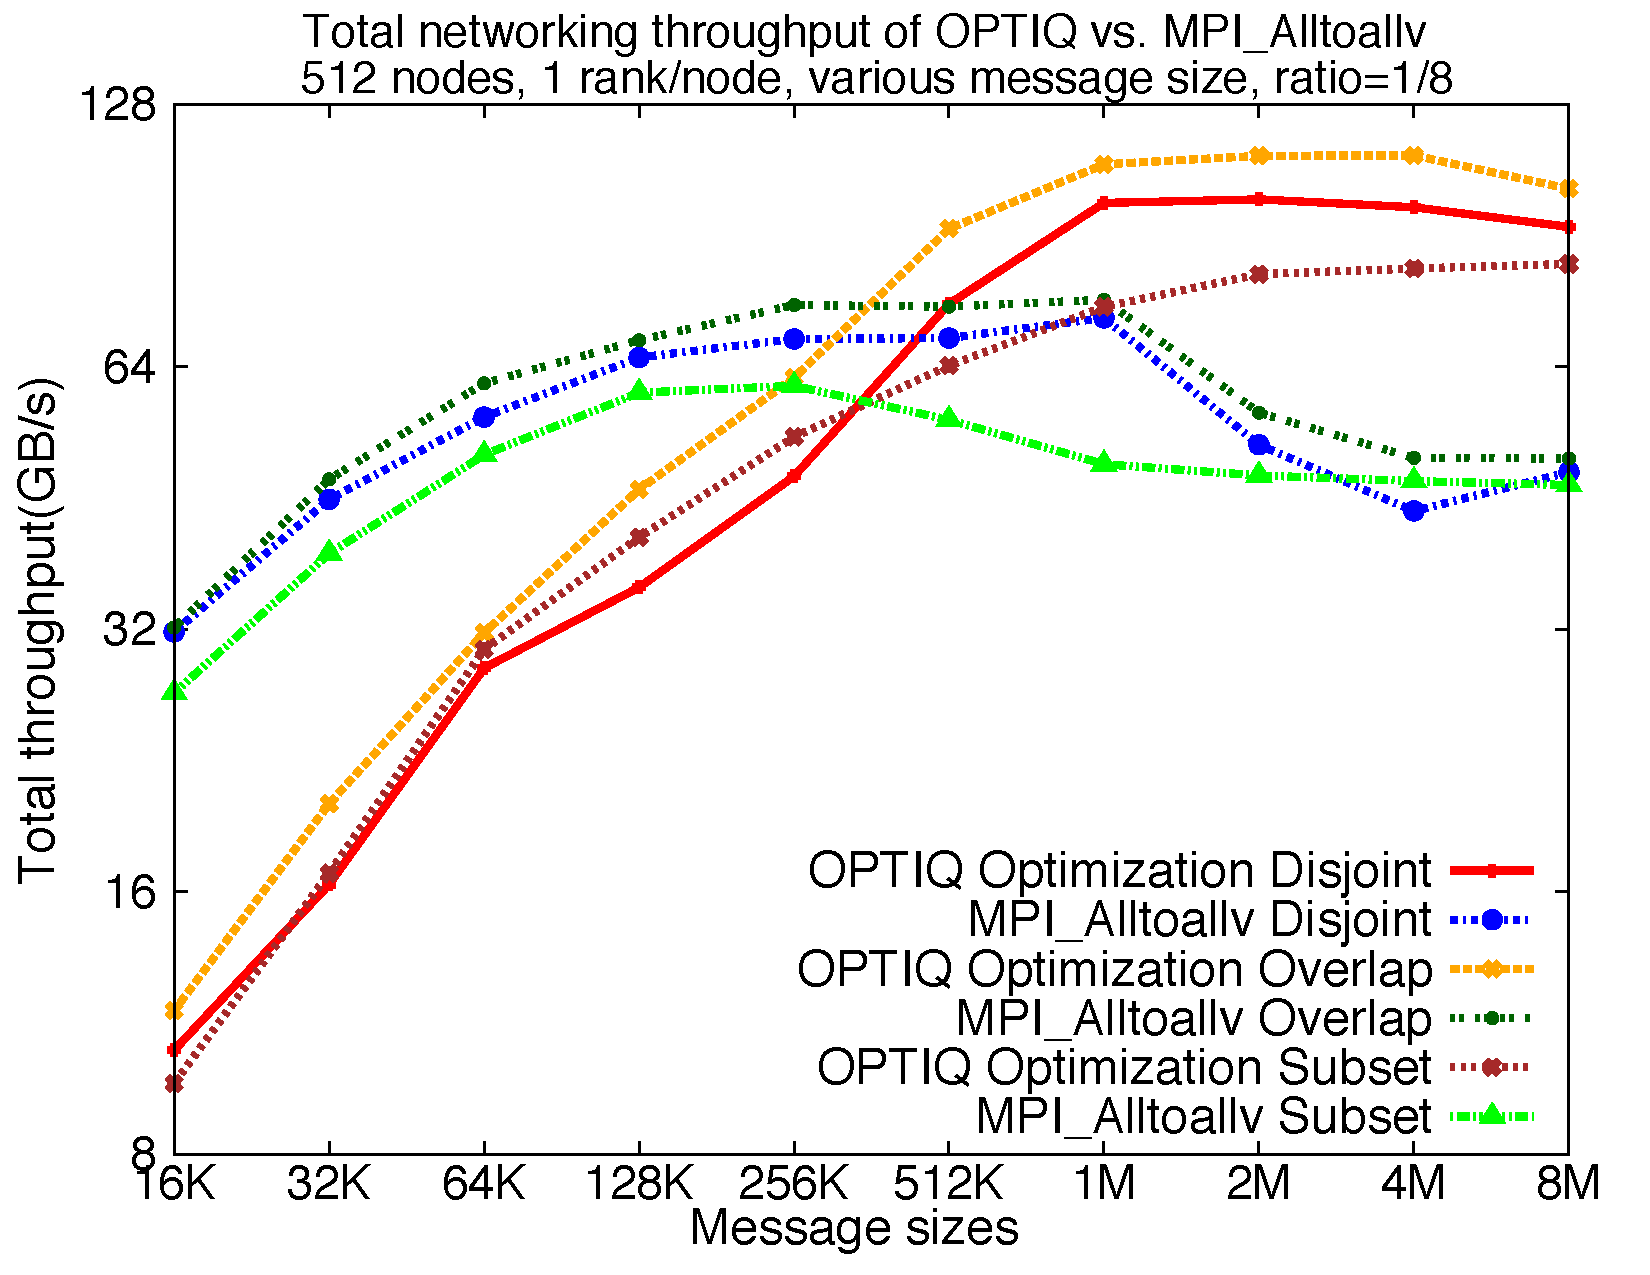
\includegraphics[scale=0.30]{figures/messagesize.pdf}
\vspace{-0.1in}
\caption{Total throughtput with different message sizes in 3 patterns.}
\vspace{-0.1in}
\label{fig:messagesize}
\end{figure}

As shown in the Figure \ref{fig:messagesize}, data transfer throughput flips at the size in between 256 KB and 512 KB. If the message size is less than 256 KB, MPI\_Alltoallv has better performance. When the message size is over 512 KB, OPTIQ has better performance. This is due to overhead caused by extra headers in each message and the time to copy and inject at each intermediate nodes.
